\newcommand{\difference}[1]{\mathrm{\Delta} #1}

\section{Einleitung}

Das LHCb-Experiment beschäftigt sich zur Überprüfung des Standardmodells mit Präzisionsmessungen an Zerfällen von \PB-Mesonen.

Eine der am LHCb-Detektor durchgeführten Messungen ist die Bestimmung der zeitabhängigen $CP$-Verletzung in den Zerfällen neutraler \PB-Mesonen.
Wichtig ist dabei die Bestimmung der Produktionzustände der erzeugten \PB-Mesonen, die als \emph{Flavour-Tagging} bezeichnet wird.
In diesem Zusammenhang muss die Fehlerrate der Tagging-Entscheidungen, auch Mistag-Wahrscheinlichkeit genannt, möglichst genau bekannt sein.

Diese Bachelorarbeit beschäftigt sich mit der \emph{Flavour-Tagging-Kalibration}, die das Ziel hat eine möglichst genaue Abschätzung der Mistag-Wahrscheinlichkeit zu liefern.
Sie basiert auf Daten des Zerfalls $\PBz \to \PJpsi\PKst$, die im Jahr 2012 aufgenommen wurden und konzentriert sich auf eine Kalibration des Same-Side-Pion-Taggers (SS$π$).
In früheren Analysen hat sich gezeigt, dass dieser ca. ein Viertel der statistischen Signifikanz aller kombinierten Tagger ausmacht.
Im Gegensatz zu anderen Taggern erlaubt er keine Kalibration mittels Zerfällen geladener \PB-Mesonen, weshalb er manuell kalibriert werden muss.

Im Folgenden soll die Konvention $\hbar = c = 1$ gelten.

\newpage

\section*{Danksagung}

Ich danke verschiedenen Leuten.

\newpage


\section{Standardmodell der Teilchenphysik}
\label{standard-model}

Das Standardmodell der Teilchenphysik ist ein Quantenfeldtheorie, die alle bislang bekannten Elementarteilchen und ihre Interaktion über die starke, schwache und elektromagnetische Wechselwirkung beschreibt.

Die Elementarteilchen lassen sich in Quarks und Leptonen (aus denen Materie besteht) und Eichbosonen (die Kräfte zwischen den Teilchen vermitteln) unterteilen.

Das Standardmodell ist ausgesprochen erfolgreich: Seine Vorhersagen decken sich mit jedem bisher durchgeführten Experiment der Hochenergiephysik.

Trotz dessen kann es sich dabei nicht um eine endgültige Theorie aller physikalischen Effekte handeln.
So gibt es noch keine allgemein akzeptierte Methode, um Gravitation in das Standardmodell mit einzubeziehen.
Außerdem ist eine Reihe von Phänomenen bekannt, die sich nicht durch das Standardmodell erklären lassen, wie das Vorhandensein und die Natur von dunkler Materie und dunkler Energie, die unerklärt hohe Materie-Antimaterie-Asymmetrie im Universum, die Existenz der Neutrinomassen, und andere.

Eine Möglichkeit Hinweise für sogenannte ,,Neue Physik'' zu finden, ist es, hochpräzise Experimente durchzuführen, die nach Abweichungen von den Vorhersagen des Standardmodells suchen.

\subsection{Quark-Sektor im Standardmodell}

Das Standardmodell beinhaltet 6 verschiedene Arten von Quarks: up, down, charm, strange, top und bottom.
Diese werden als \Pqu, \Pqd, \Pqc, \Pqs, \Pqt und \Pqb abgekürzt und häufig auf folgende Art in drei Familien unterteilt:
\begin{eqn}
  \begin{pmatrix}
    \Pqu & \Pqc & \Pqt \\
    \Pqd & \Pqs & \Pqb \\
  \end{pmatrix}
  \eqlabel{quarks}
\end{eqn}
Alle 6 sogenannten Quark-Flavour besitzen unterschiedliche Massen.

Ein erster experimenteller Beleg für die Existenz von Quarks wurde 1969 am Stanford Linear Accelerator (SLAC) durch Elektron-Streuexperimente (Deep Inelastic Scattering) an Protonen demonstriert werden.\cite{slac-quarks}

Quarks besitzen eine elektrische Ladung, wechselwirken also elektromagnetisch.
Up-artige Quarks (die obere Reihe in \eqref{quarks}) besitzen eine Ladung von $⅔$ der Elementarladung, down-artige Quarks (die untere Reihe) eine Ladung von $-⅓$ der Elementarladung.
Neben jedem der Quarks existiert ein Antiquark mit gleicher Masse aber umgekehrter Ladung.

Quarks sind die einzigen bekannten Elementarteilchen, die an die starke Wechselwirkung koppeln.
Jedes Quark besitzt dazu eine sogenannte Farbladung.
Beobachtet werden können nur gebundene Quark-Zustände, deren Farbladungen sich zu Null addieren.

Quarks nehmen zusätzlich noch an der schwachen Wechselwirkung teil.
Im Gegensatz zur elektromagnetischen und starken Wechselwirkung erhält diese nicht den Quark-Flavour.
So kann ein Quark unter Abgabe eines \PW-Bosons seine Zeile in \eqref{quarks} ändern.
Dabei bleibt es mit hoher Wahrscheinlichkeit in derselben Spalte.
Ein Wechsel der Spalte ist allerdings nicht ausgeschlossen.
Dieser Mechanismus lässt sich über die Cabibbo-Kobayashi-Maskawa-Matrix (CKM-Matrix) wie folgt ausdrücken.
\begin{eqn}
  \begin{pmatrix}
    $\Pqd'$ \\
    $\Pqs'$ \\
    $\Pqb'$ \\
  \end{pmatrix}
  =
  \begin{pmatrix}
    V_{\Pqu\Pqd} & V_{\Pqu\Pqs} & V_{\Pqu\Pqb} \\
    V_{\Pqc\Pqd} & V_{\Pqc\Pqs} & V_{\Pqc\Pqb} \\
    V_{\Pqt\Pqd} & V_{\Pqt\Pqs} & V_{\Pqt\Pqb} \\
  \end{pmatrix}
  \begin{pmatrix}
    \Pqd \\
    \Pqs \\
    \Pqb \\
  \end{pmatrix}
\end{eqn}
Sie übersetzt die Flavor-Eigenzustände 
\begin{eqn}
  \begin{pmatrix}
    \Pqu \\  
    \Pqd \\  
  \end{pmatrix}
  ,
  \begin{pmatrix}
    \Pqc \\ 
    \Pqs \\ 
  \end{pmatrix}
  ,
  \begin{pmatrix}
    \Pqt \\ 
    \Pqb \\ 
  \end{pmatrix}
\end{eqn}
in Eigenzustände der schwachen Wechselwirkung
\begin{eqn}
  \begin{pmatrix}
    \Pqu \\  
    $\Pqd'$ \\  
  \end{pmatrix}
  ,
  \begin{pmatrix}
    \Pqc \\ 
    $\Pqs'$ \\ 
  \end{pmatrix}
  ,
  \begin{pmatrix}
    \Pqt \\ 
    $\Pqb'$ \\
  \end{pmatrix}\:.
\end{eqn}

Die CKM-Matrix muss unitär sein, da sie lediglich eine Rotation der Eigenzustände darstellt.

Im Folgenden soll auf den Begriff der $CP$-Verletzung näher eingegangen werden.

\subsection{$CP$-Verletzung im Standardmodell}

\newcommand{\Vud}{V_{\Pqu\Pqs}}
\newcommand{\Vus}{V_{\Pqu\Pqs}}
\newcommand{\Vub}{V_{\Pqu\Pqb}}
\newcommand{\Vcd}{V_{\Pqc\Pqd}}
\newcommand{\Vcs}{V_{\Pqc\Pqs}}
\newcommand{\Vcb}{V_{\Pqc\Pqb}}
\newcommand{\Vtd}{V_{\Pqt\Pqd}}
\newcommand{\Vts}{V_{\Pqt\Pqs}}
\newcommand{\Vtb}{V_{\Pqt\Pqb}}

Drei diskrete Symmetrieoperatoren sind im Standardmodell von Interesse:
Der Ladungskonjugations-Operator $C$, der Teilchen in ihre Antiteilchen transformiert und umgekehrt.
Der Paritätsoperator $P$, der das System in allen drei Raumachsen spiegelt.
Der Zeitumkehroperator $T$, der den Zeitfluss des Systems umkehrt.

Lange Zeit dachte man, dass die Physik unter Anwendung von $P$ invariant bliebe.
Ein 1956 von Lee und Yang postuliertes \cite{cp-lee-yang} und von Wu durchgeführtes \cite{wu} Experiment zeigt aber, dass dies nicht der Fall ist.

Daraufhin nahm man an, dass die Kombination aus Ladungskonjugation und Paritätsumkehr, $CP$, eine universelle Symmetrie darstellen würde.
Doch auch das konnte anhand des neutralen Kaon-Systems von Cronin, Fitch, u.a 1964 widerlegt werden\cite{kaons-cronin-fitch}.
$CP$-Verletzung wurde ausschließlich in hadronischen Systemen beobachtet.

Sie ist im Standardmodell als komplexe Phase in der CKM-Matrix verwirklicht.
Die Tatsache, dass dieser Mechanismus nur bei Existenz von mindestens drei Quarkfamilien funktioniert, inspirierte Kobayashi und Maskawa 1973 dazu, die Existenz der damals noch nicht entdeckten dritten Quarkfamilie (top und bottom) zu postulieren.
Dafür erhielten beide 2008 den Nobelpreis.

Eine Möglichkeit die in der CKM-Matrix kodierte $CP$-Verletzung zu visualisieren sind die sogenannten Unitaritätsdreiecke.
Hierzu bildet man einzeln die Produkte der Spalten der CKM-Matrix, sowie die der Zeilen.
Da die CKM-Matrix zwingend unitär sein muss, folgt für 6 der Produkte, dass sie $0$ ergeben müssen.

Die Produkte bestehen jeweils aus drei komplexen Termen:
\begin{eqn}
  \Vud\Vub^* + \Vcd\Vcb^* + \Vtd\Vtb^* = 0
\end{eqn}
Die 3 Terme können als Linien in der komplexen Ebene interpretiert werden, die sich zu einem Dreieck schließen.
Nützlich ist es, jede der Seiten auf $\Vcd\Vcb^*$ zu normieren; der einzige freie Parameter ist dann die Lage der Dreiecks-Spitze (siehe Abb. \ref{unitarity-triangle}).

\begin{figure}
  \centering
  \begin{tikzpicture}[scale=6]
    \coordinate (A) at (0.225,0.345);
    \coordinate (B) at (1,0);
    \coordinate (C) at (0,0);

    \draw (A) -- node[above right] {$\abs{\frac{\Vtd \Vtb^*}{\Vcd \Vcb^*}}$} (B) -- node[below] {$1$} (C) -- node[above left] {$\abs{\frac{\Vud \Vub^*}{\Vcd \Vcb^*}}$} (A);

    \begin{scope}
      \path[clip] (A) -- (B) -- (C) -- cycle;
      \draw (A) circle (0.17);
      \draw (B) circle (0.3);
      \draw (C) circle (0.19);
    \end{scope}

    \node at (0.240,0.260) {$α$};
    \node at (0.77,0.045) {$β$};
    \node at (0.10,0.06) {$γ$};

  \end{tikzpicture}
  \caption{Das Unitaritätsdreieck $\Vud\Vub^* + \Vcd\Vcb^* + \Vtd\Vtb^* = 0$ mit Seitenlängen normiert auf $\Vcd\Vcb^*$.
  Das transformierte Dreieck lässt ist vollständig durch die Lage der Dreiecks-Spitze festgelegt.}
  \label{unitarity-triangle}
\end{figure}

Interessant ist, dass die somit vom Standardmodell vorhergesagte CP-Verletzung sich mit jedem bisherigen Experiment gedeckt hat, obwohl die vorhergesagte Menge nicht dazu in der Lage ist die im Universum beobachtete Materie-Antimaterie Asymmetrie zu erklären.

Eine Möglichkeit den CKM-Mechanismus auf seine Gültigkeit zu überprüfen, ist durch Durchführen mehrerer Experimente Grenzen für die Lage der Dreiecks-Spitze aus Abb. \ref{unitarity-triangle} zu bestimmen, sie sogar regelrecht überzubestimmen.
Widersprüche oder Abweichungen von der Theorie würden dann z.B. darauf hindeuten, dass es weitere Elementarteilchen geben könnte, die im CKM-Mechanismus nicht beachtet wurden, oder sogar insgesamt seine Gültigkeit in Frage stellen.

In diesem Zusammenhang wurden zahlreiche Experimente durchgeführt.
Ein äußerst aussagekräftiges Experiment ermöglicht die Bestimmung des Winkels $β$ und basiert auf der Oszillation neutraler \PB-Mesonen.

\subsection{$\PB$-$\PaB$-Oszillation}

Als \PB-\PaB-Oszillation bezeichnet man die Tatsache, dass neutrale \PB-Mesonen bei freier Propagation je nach Lebensdauer eine bestimmte Wahrscheinlichkeit haben als ihr Antiteilchen zu zerfallen.
Die Oszillation neutraler Mesonen war bereits von Cronin und Fitch im Kaon-System verwendet worden, um $CP$-Verletzung zu demonstrieren\cite{kaons-cronin-fitch}.
Dass auch neutrale $B$-Mesonen eine Oszillation aufweisen, wurde 1987 von der Argus-Kollaboration am DESY gezeigt\cite{argus-bbar}.

Dass Amplituden für die Übergänge eines $\PBz$ zu seinem Antiteilchen und umgekehrt existieren, lässt sich anhand der beiden Feynman-Diagramme in Abb. \ref{bbar-oscillation} verstehen.

\begin{figure}
  \begin{tikzpicture}[line width=1.2 pt, scale=1.1]
    \draw[fermion] (-1,2.3) node [left] {\Pqd} -- (0,2);
    \draw[fermion] (0,2) -- node [above] {$\Pqu,\Pqc,\Pqt$} (2, 2);
    \draw[fermion] (2,2) -- (3,2.3) node [right] {\Pqb};
     
    \draw[fermionbar] (-1,-.3) node [left] {\Pqb} -- (0,0);
    \draw[fermionbar] (0,0) -- node [above] {$\Pqu,\Pqc,\Pqt$} (2,0);
    \draw[fermionbar] (2,0) -- (3,-.3) node [right] {\Pqd};
    
    \draw[vector] (0,2) -- node [left] {\PW} (0,0);
    \draw[vector] (2,2) -- node [right] {\PW} (2,0);
  \end{tikzpicture}
  \hspace{1cm}
  \begin{tikzpicture}[line width=1.2 pt, scale=1.1]
    \draw[fermion] (-1,2.3) node [left] {\Pqd} -- (0,2);
    \draw[vector] (0,2) -- node [above] {\PWm} (2, 2);
    \draw[fermion] (2,2) -- (3,2.3) node [right] {$b$};
     
    \draw[fermionbar] (-1,-.3) node [left] {\Pqb} -- (0,0);
    \draw[vector] (0,0) -- node [above] {\PWp} (2,0);
    \draw[fermionbar] (2,0) -- (3,-.3) node [right] {\Pqd};
    
    \draw[fermion] (0,2) -- node [left] {$\Pqu,\Pqc,\Pqt$} (0,0);
    \draw[fermionbar] (2,2) -- node [right] {$\Pqu,\Pqc,\Pqt$} (2,0);
  \end{tikzpicture}
  \label{bbar-oscillation}
  \caption{Feynman-Diagramme der \PBz-\PaBz-Oszillation.
  In dieser Ordnung ergibt sich die Amplitude für einen Flavour-Wechsel als Summe beider Diagramme.}
\end{figure}

Im Folgenden sollen die Übergangswahrscheinlichkeiten für $\PBz \to \PBz$ und $\PBz \to \PaBz$ bestimmt werden.
Die Herleitung orientiert sich an \ref{babar-book} und an einer Vorlesung von B. Spaan.

Zu jedem Zeitpunkt lässt sich der Zustand des \PBz-\PaBz-Systems als
\begin{eqn}
  ψ = a \ket{\PBz} + b \ket{\PaBz}
\end{eqn}
schreiben.
Der zugehörige Hamiltonian, der Zerfall und Übergang der beiden Zustände beschreibt, ist durch
\begin{eqn}
  H = 
  \begin{pmatrix}
    M_{11}-\frac{\I}{2} Γ_{11} & M_{12}-\frac{\I}{2} Γ_{12} \\
    M^*_{12}-\frac{\I}{2} Γ^*_{12} & M_{22}-\frac{\I}{2} Γ_{22} \\
  \end{pmatrix}
\end{eqn}
gegeben.
Durch Diagonalisierung von $H$ erhält man die Eigenzustände
\begin{eqns}
  B_L &=& p \ket{\PBz} + q \ket{\PaBz} \\
  B_H &=& p \ket{\PBz} - q \ket{\PaBz}
\end{eqns}
mit
\begin{eqn}
  \frac{q}{p} = \frac{\difference{m_{\Pqd}} - \frac{\I}{2}\difference{Γ_{\Pqd}}}{2M_{12} - \frac{\I}{2}\difference{Γ_{\Pqd}}}\:.
\end{eqn}
Dabei ist $\difference{m_{\Pqd}}$ der Unterschied $M_H - M_L$ zwischen den Massen der beiden Eigenzuständen und $\difference{Γ_{\Pqd}}$ die Differenz ihrer Zerfallsbreiten.
Wie auf den Seiten 8 und 9 in \ref{babar-book} begründet, lassen sich folgende Näherungen machen:

% ...

\begin{eqns}
  \ket{\PBz(t)} &=& g_+(t) \ket{\PBz} + \frac{q}{p} g_-(t)\ket{\PaBz} \\
  \ket{\PaBz(t)} &=& \frac{q}{p} g_-(t) \ket{\PBz} + g_+(t)\ket{\PaBz}
\end{eqns}
mit
\begin{eqns}
  g_+(t) &=& \E^{-\I M t} \E^{-½Γt} \cos(Δm_{\Pqd} t/2) \\
  g_-(t) &=& \E^{-\I M t} \E^{-½Γt} \I\sin(Δm_{\Pqd} t/2)
\end{eqns}

Die gesuchten Wahrscheinlichkeiten, dass ein Meson seinen Flavour geändert oder nicht geändert hat, ergeben sich dann als die Übergangswahrscheinlichkeiten von einem Zustand zum anderen:
\begin{eqn}
  \braket{\PaBz(t)}{\PBz(0)}^2 = \braket{\PBz(t)}{\PaBz(0)}^2 = \frac{1}{4} (\E^{-Γ_Lt} + \E^{-Γ_Ht} + 2\E^{-\frac{Γ_L + Γ_H}{2}t} \cos(\difference{m_{\Pqd}}t)
\end{eqn}
\begin{eqn}
  \braket{\PBz(t)}{\PBz(0)}^2 = \braket{\PaBz(t)}{\PaBz(0)}^2 = \frac{1}{4} (\E^{-Γ_Lt} + \E^{-Γ_Ht} - 2\E^{-\frac{Γ_L + Γ_H}{2}t} \cos(\difference{m_{\Pqd}}t)
\end{eqn}

% Berechnung der Mixing-Asymmetrie: (A - B) / (A + B)
% Mixing: q

\begin{eqn}
  M_\t{sig}(t) = \frac{N_{q=1}(t) - N_{q=-1}(t)}{N_{q=1}(t) + N_{q=-1}(t)} = \cos(\difference{m_{\Pqd}} t)
  \label{mixing}
\end{eqn}

%\cite{pdg}

% 3 Arten von CP-Verletzung?

% B⁰ → J/ψ K*
%\begin{tikzpicture}[line width=1.2 pt, scale=2]
%  \draw[fermion] (0, 0.5) node [left] {\Pqd} -- (2, 0.5) node [right] {\Pqd};
%  \draw[fermionbar] (0, 0) node [left] {\Pqb} -- (0.75, 0);
%  \draw[fermionbar] (1.25, 0) -- (2, 0) node [right] {\Pqs};
%  \draw[vector] (0.75, 0) -- node [above] {\PW} (1.25, 0);
%  \draw[fermion] (1.25, 0) -- (2, -0.5) node [below] {\Pqc};
%  \draw[fermionbar] (0.75, 0) -- (1.500, -0.5) node [below] {\Pqc};
%\end{tikzpicture}

\Comment{Clean up this mess.}

\section{Experimentelle Grundlagen}

\subsection{Der LHCb-Detektor}

Der Large Hadron Collider beauty Detektor (LHCb) ist eines der vier größten Experimente, die am Large Hadron Collider (LHC) in Genf durchgeführt werden.

Er wurde vorranging gebaut, um die Zerfälle von \PB-Mesonen auf Hinweise für neue Physik zu untersuchen.

Im Gegensatz zu den anderen großen Detektoren am LHC (ATLAS, ALICE und CMS) handelt es sich hierbei nicht um einen $4π$-Detektor, sondern um ein einarmiges Vorwärts-Spektrometer mit einer Winkelakzeptanz von lediglich $10$ bis \SI{300}{\radian}.
Er ist für eine vergleichsweise geringe Luminosität, gleichzeitig aber für eine hochpräzise Rekonstruktion ausgelegt.

Die folgenden Informationen sind \cite{lhcb} entnommen.
Ein Querschnitt des Detektors ist in \ref{lhcb} dargestellt.

Der Detektor ist über die sogenannte \emph{Beampipe} an den LHC angeschlossen.

Der \emph{Vertex Locator} (VELO) ist ein Siliziumdetektor, der aus 2 Hälften besteht und bis auf \SI{5}{\milli\metre} an den Protonenstrahl herangefahren werden kann. Er wird zur Vertex-Rekonstruktion und zur Auflösung der Impact Parameter verwendet. Er ist in der Lage Entfernungen von \SI{10}{\micro\metre} aufzulösen.

Die beiden Ring Imaging Cherenkov (RICH) Detektoren messen mittels Cherenkov-Strahlung die Geschwindigkeit geladener Teilchen, was durch Vergleich mit Informationen aus dem Tracking eine Bestimmung der Teilchen-Massen erlaubt und damit zusammen mit der Information über die Ladung des Teilchens seine Identifizierung (PID) ermöglicht.

Der konventionelle (nicht-supraleitende) Dipolmagnet verfügt über ein integriertes Magnetfeld von \SI{4}{\tesla\metre}.

Die Trackerstationen T1 bis T3 ermöglichen eine Verfolgung der Teilchenbahnen.

Dahinter befinden sich die elektromagnetischen und hadronischen Kalorimeter, die Elektronen, Photonen und Hadronen auffangen und ihre Energie messen.

Am Ende des Detektors befindet sich eine Reihe von Drahtkammern, die eine Identifikation von Muonen ermöglichen.

\begin{figure}
  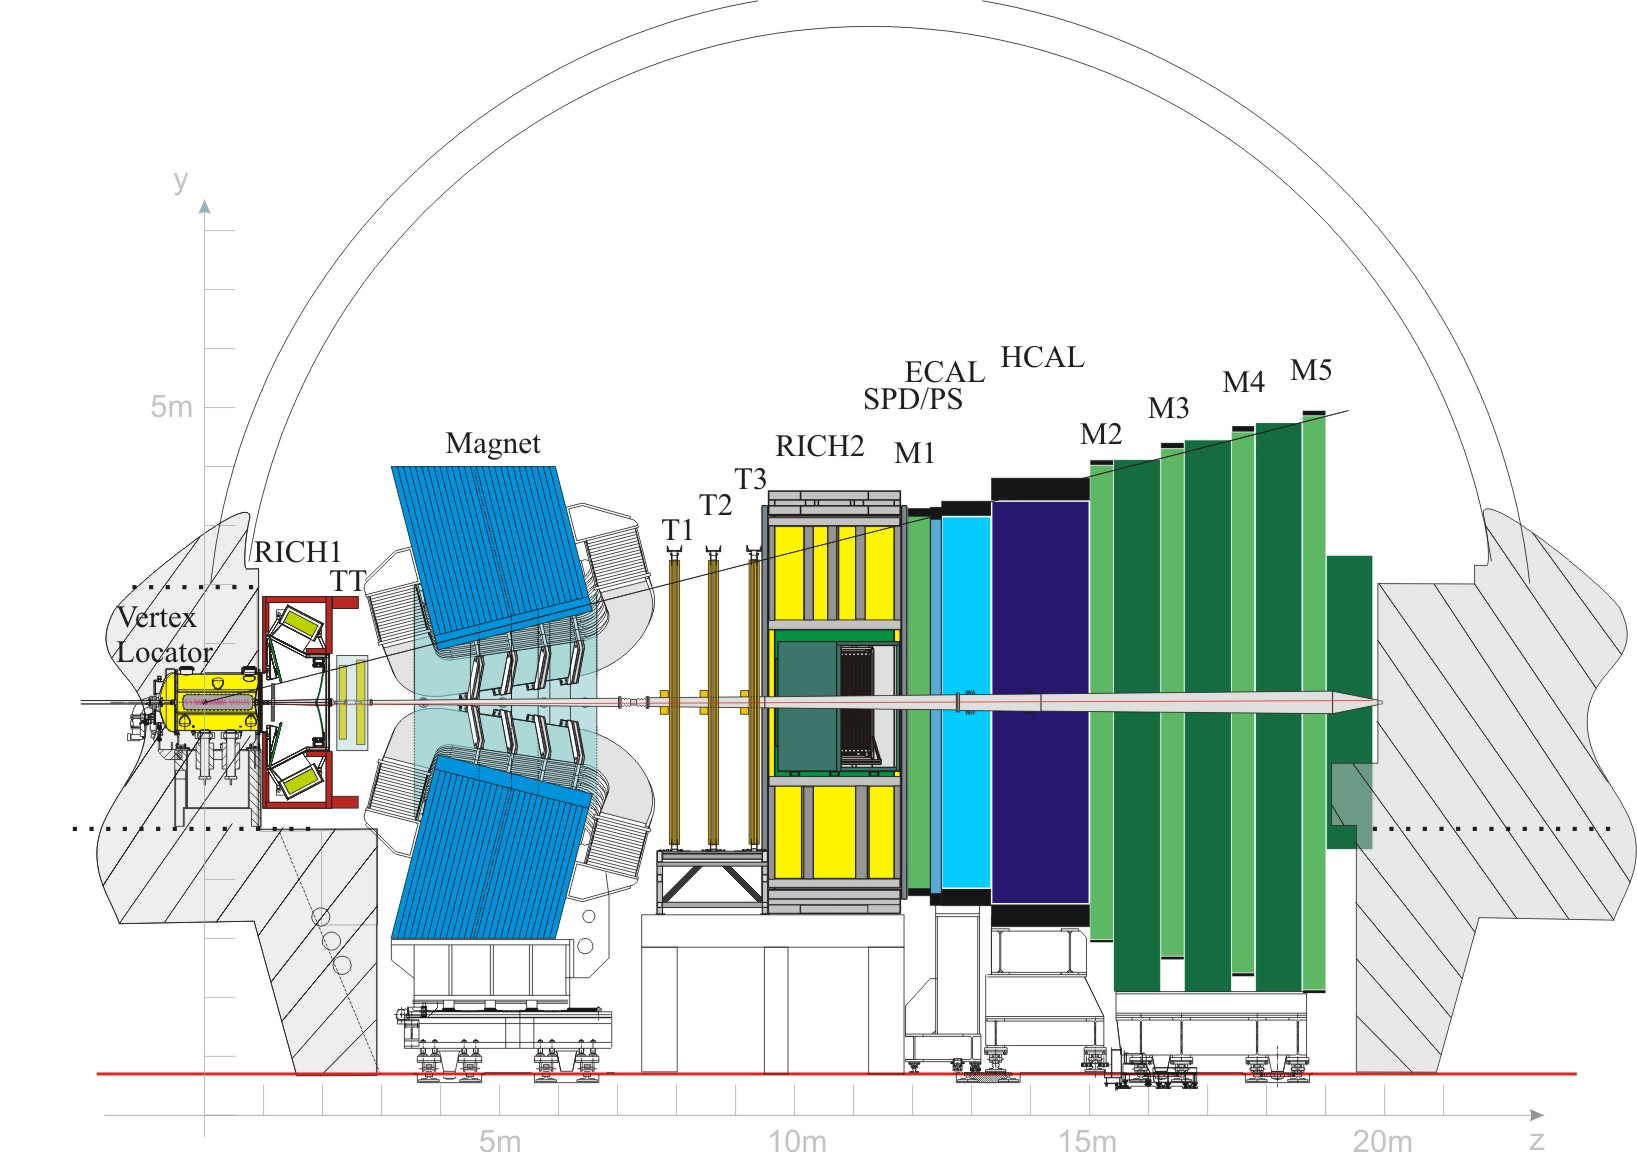
\includegraphics[width=\textwidth]{figures/lhcb.pdf}
  \caption{Querschnitt des LHCb-Detektors. Die einzelnen Komponenten werden im Text erläutert.\cite{lhcb}}
  \label{lhcb}
\end{figure}

\subsection{Flavour-Tagging}

Zur Bestimmung der Oszillationsfrequenz $\difference{m_{\Pqd}}$ der produzierten $\PB$- und $\PaB$-Mesonen muss neben den Lebensdauern der einzelnen beobachteten Mesonen sowohl deren End-, als auch deren Anfangszustand bekannt sein.

Der Endzustand kann aus den Zerfallsprodukten der \PBz und \PaBz Mesonen bestimmt werden, wenn man einen Kanal mit self-tagging Endzustand wählt.
Zu diesen Kanälen gehören $\PBz \to \PDm \Pgpp$ und $\PBz \to \PJpsi \PKst$ (und die entsprechenden ladungskonjugierten Kanäle).

Die Bestimmung des Anfangszustandes, die man als \emph{Flavour-Tagging} bezeichnet, erweist sich als deutlich schwieriger.
Das LHCb-Experiment verwendet hierzu neuronale Netze, die darauf trainiert werden unter Einbeziehung weiterer, während des Events erfolgter, Beobachtungen eine möglichst gute Abschätzung für den Typ des \PB-Mesons (den sogenannten \emph{Tag}) zu liefern.

Die verwendeten Tagger lassen sich in zwei Typen unterteilen: Opposite-Side-Tagger (OST) und Same-Side-Tagger (SST).

\begin{figure}
  \centering
  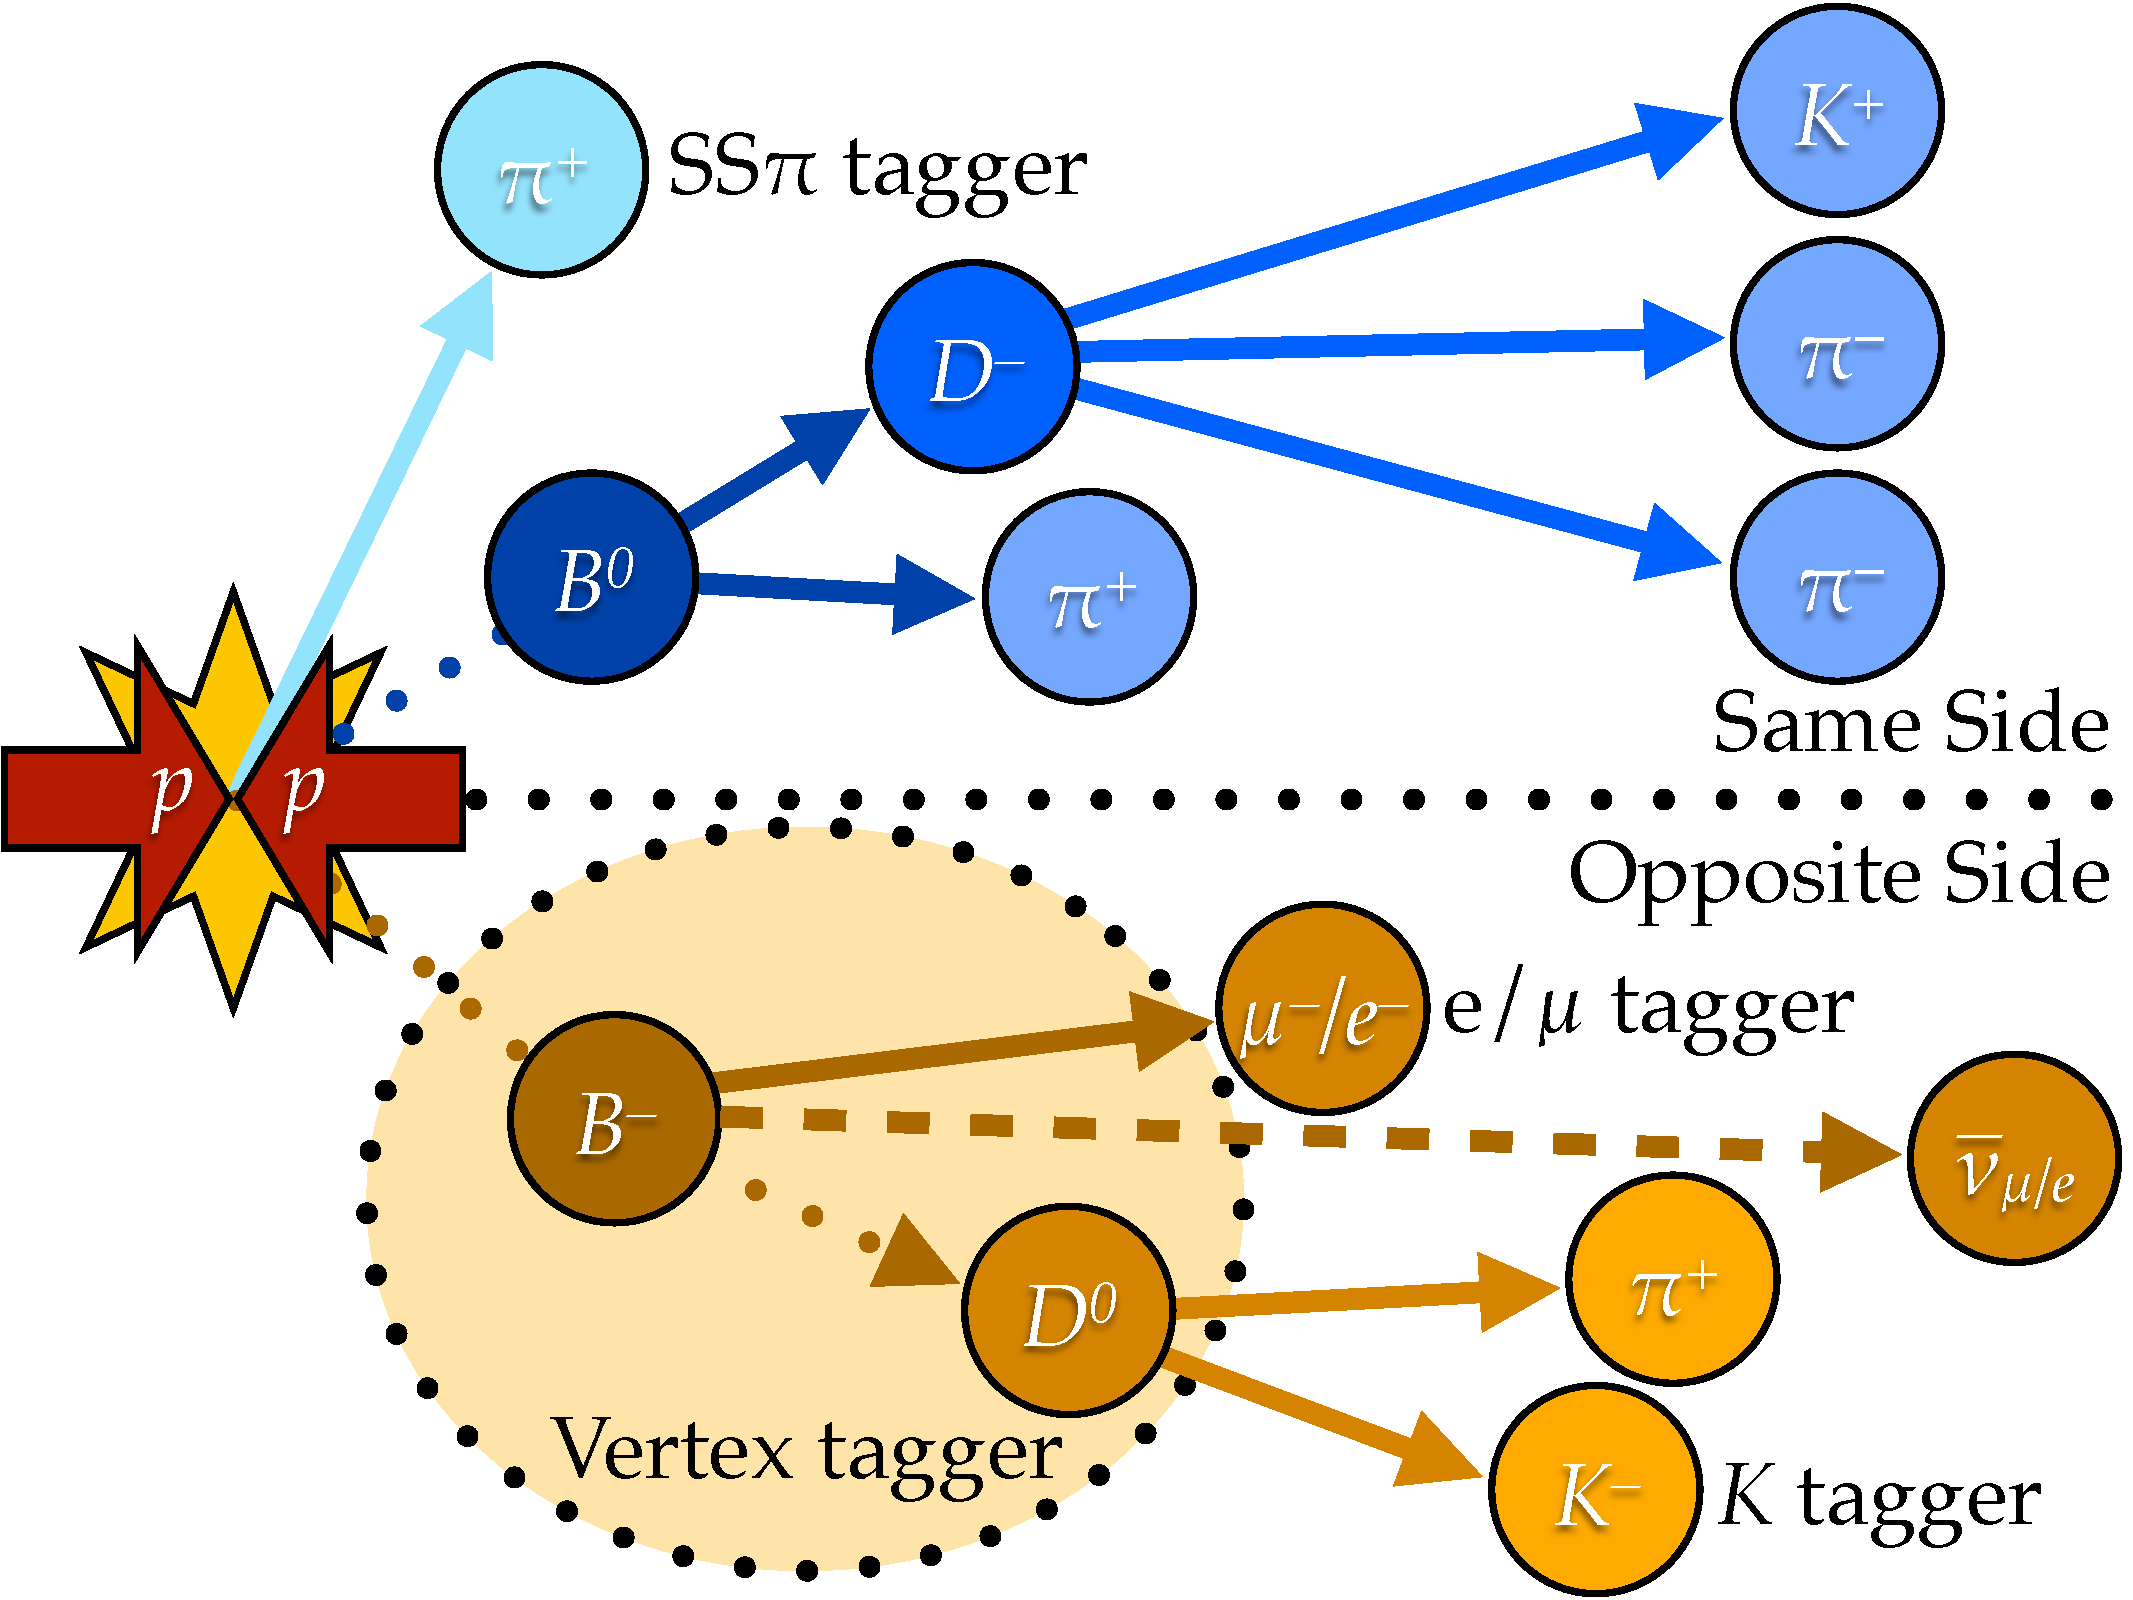
\includegraphics[width=0.6\textwidth]{figures/tagging.pdf}
  \caption{Funktionsweise der Same-Side-Tagger (oben) und der Opposite-Side-Tagger (unten). Oben lässt sich aus der Ladung eines neben dem \PB-Meson entstandenen Pions auf den Quarkinhalt des \PB schließen. Unten wird genutzt, dass das ebenfalls entstandene \Pqb-Quark ein geladenes \PBm gebildet hat, dessen Ladung sich aus den Zerfallsprodukten rekonstruieren lässt.}
  \label{tagging}
\end{figure}

Die Opposite-Side-Tagger (OST) basieren auf der Tatsache, dass \Pqb-Quarks fast ausschließlich als \Pqb\Paqb-Paar entstehen. Bildet dann z.B. das \Pqb-Quark ein \PaB-Meson, so könnte das ebenfalls entstandene \Paqb ein geladenes Meson, nämlich ein \PBp bilden, dessen Zerfallsprodukte einen Rückschluss auf seine Ladung und damit indirekt auf den Quarkinhalt des \PaB-Mesons ermöglichen.
So kann das geladene \PB-Meson z.B. semileptonisch ($\Pqb \to \Pqc \Plepton \APnulepton$) zerfallen. Die Ladung des Leptons entspricht dann (bei Vernachlässigung der selteneren Zerfallsreihe $\Pqb \to \Pqc \to \Pqs \APlepton \Pnulepton$) der gesuchten Mesonladung, die eine Bestimmung des \PB-Flavours erlaubt.\cite{ost}
Der Vorgang ist in der unteren Hälft von Abbildung \ref{tagging} gezeigt.

Die Same-Side-Tagger (SST) basieren auf der Betrachung von Hadronisierungsprozessen bei der Entstehung des \PB-Mesons.
Ein entstandenes \Pqb-Quark benötigt zur Bildung eines \APB ein \APqd-Quark.
Dieses ist zusammen mit einem \Pqd entstanden, welches wiederum ein Hadron bildet, z.B. ein Pion oder Kaon.
Ist dieses geladen, so lässt sich aus der Ladung des Pions oder Kaons auf den Typ des \Pqd-Quarks im \PB-Meson schließen und damit sein Produktionszustand bestimmen.
Die Funktionsweise ist in der oberen Hälfte von Abbildung \ref{tagging} abgebildet.

Die so ermittelte Tag-Entscheidung ist nicht immer richtig; die Wahrscheinlichkeit, dass sie falsch ist bezeichnet man als Mistag-Wahrscheinlichkeit $ω$.
Sie kann zwischen $0$ (immer korrekt) und $0.5$ (zufällige Entscheidung) liegen.
Werte zwischen $0.5$ und $1$ sind auch zulässig, man könnte die Mistag-Wahrscheinlichkeit dann aber durch Umdrehen aller Tag-Entscheidungen wieder in das erste Intervall umklappen.

Die Mistag-Wahrscheinlichkeit taucht bei einer Bestimmung von $\difference{m_{\Pqd}}$ als Parameter auf, da sie die Amplitude der Mixing-Verteilung \eqref{mixing} verringert.
Dies lässt sich wie folgt verstehen:
Wird den zerfallenen Mesonen mit der Wahrscheinlichkeit $ω$ der falsche Tag  zugeordnet, so setzen sich die gemessenen Anzahlen von gemischten und ungemischten Ereignissen pro Zeitintervall über
\begin{eqns}
  N_{q=1,\t{measured}} &=& (1-ω) N_{q=1} + ω N_{q=-1} \\
  N_{q=-1,\t{measured}} &=& (1-ω) N_{q=-1} + ω N_{q=1}
\end{eqns}
zusammen.

Nach Einsetzen in \eqref{mixing} ergibt sich also
\begin{eqns}
  M_\t{sig} &=& \frac{(1-ω) N_{q=1} + ω N_{q=-1} - (1-ω) N_{q=-1} - ω N_{q=1}}
                     {(1-ω) N_{q=1} + ω N_{q=-1} + (1-ω) N_{q=-1} + ω N_{q=1}} \\
            &=& (1-2ω) \frac{N_{q=1} - N_{q=-1}}{N_{q=1} + N_{q=-1}} \\
            &=& (1-2ω) \cos(\difference{m_{\Pqd}} t)
  \label{mixing}
\end{eqns}
Den Faktor $D = 1 - 2ω$ bezeichnet man als \emph{Dilution}.

Zur Bewertung des Taggings lässt sich die Tagging-Effizienz $ε_\t{tag}$ einführen.
Diese ist einfach das Verhältnis zwischen der Anzahl der getaggten und aller Signalereignisse.
Darüber lässt sich eine effektive Effizienz oder Tagging-Power als $ε_\t{eff} = ε_\t{tag} D^2$ definieren.
Diese macht eine Aussage über die statistische Genauigkeit des Tagging-Samples.

Wichtig ist eine genaue Kenntnis von $ω$ beispielsweise bei einer Messung der zeitabhängigen CP-Verletzung in der Oszillation neutraler \PB-Mesonen.
Hier misst man auf einem Kanal, der zwar nicht über einen self-tagging Endzustand verfügt, bei dem aber die Wahrscheinlichkeit, dass ein entstandenes Meson im Zustand \PBz oder \PaBz zerfällt eine in der Zeit oszillierende Asymmetrie aufweist.
Die CP-Verletzung ist hier also für die Amplitude der beobachteten Oszillation verantwortlich.
Von kritischer Bedeutung für die Messung ist es daher, alle Faktoren, die die gemessene Amplitude beeinflussen, möglichst präzise zu bestimmen.
Dazu gehört neben der Zeitauflösung in erster Linie die Mistag-Wahrscheinlichkeit.

Da ein direkter Fit der Mistag-Wahrscheinlichkeit, anders als bei einem Kanal mit self-tagging Endzustand, hier nicht möglich ist, muss ein anderer Weg gefunden werden, um eine möglichst präzise Abschätzung von $ω$ zu erhalten.
Die verwendeten neuronalen Netze geben hierzu für jedes getaggte Event einen Mistag-Wert $η$ aus.
Dieser entspricht in der Regel aber nicht $ω$, sondern muss auf den betrachteten Zerfallstyp angepasst werden.
Durch einen $\difference{m_{\Pqd}}$-Fit lässt sich eine direkte Gegenüberstellung des tatsächlichen (gefitteten) $ω$ und der Abschätzung $η$ erzeugen.
Dieser Zusammenhang kann z.B. durch einen linearen Fit effektiv parametrisiert werden.
Das so gewonnene $ω(η)$ erlaubt es, zu einem späteren Zeitpunkt $η$ zu einer korrigierten Abschätzung $η_C$ umzurechnen.
Diesen Vorgang bezeichnet man als \emph{Tagging-Kalibration}.

\section{Datensatz}
\label{datensatz}

Der verwendete Datensatz enthält $\PBzero \to \PJpsi\PKst$-Ereignisse, im Zeitraum 2012 aufgenommen wurden.

Er beinhaltet ca. $5\cdot10^5$ Events, die bei einer integrierten Luminosität von $2$\:fb$^-1$, einer Schwerpunktsenergie von \SI{7}{\tera\electronvolt} und einem Bunch-Spacing von \SI{50}{\nano\second} detektiert wurden.

Es wurde eine auf Boosted Decision Trees (BDT) basierte Selektion durchgeführt.
Die dabei bestimmten Cut-Parameter sind noch nicht veröffentlicht.

\section{\texorpdfstring{Kalibration des $SS\pi$-Taggers für $\PBzero \to \PJpsi \PKst$}{Kalibration des SSpi-Taggers für B0 -> JpsiKst}}

Das erste Ziel der vorliegenden Analyse ist es, eine Kalibration des Same-Side-Pion-Taggers auf dem in Kapitel \ref{datensatz} beschriebenen Datensatz durchzuführen.
Das zweite Ziel ist ein Wiederholen der Analyse auf einer Version des beschriebenen Datensatzes, die mittels einer aus $\PBz \to \PDm\Pgpp$-Zerfällen gewonnenen Kalibrationsparametrisierung kalibriert wurde.

Aus einer bisherigen Analyse ist bekannt, dass der SS$π$-Tagger ca. \SI{25}{\percent} der Tagging-Power bei der Bestimmung von $\sin(2β)$ ausmacht.

Zur Kalibration wird der Datensatz je nach Größe der Mistag-Vorhersage $η$ des neuronalen Netzes in fünf Kategorien aufgeteilt.
Das mittlere $η$ wird jeweils für alle Signalereignisse pro Kategorie ermittelt.
Die Trennung von Signal und Untergrund erfolgt hierbei über das sPlot-Verfahren\cite{splot}, wobei ausschließlich die Massenverteilung zur Unterscheidung von Signal und Untergrund verwendet wird.

Aus dem Datensatz bekannt sind die Massen- und Zerfallszeit-Verteilungen der rekonstruierten \PB-Mesonen, die Tag-Entscheidung des neuronalen Netzes sowie die Kenntnis über die Kaon-Ladung, die eine Identifizierung des Endzustandes erlaubt (Das \PKst zerfällt in \PKp\Pgpm).

Aus der Tag-Entscheidung und dem Endzustand lässt sich bestimmen, ob (bei korrektem Tag) ein Wechsel des \Pqb-Flavours stattgefunden hat.
Mittels dieser Informationen kann ein zweidimensionaler, simultaner Extended-Maximum-Likelihood-Fit über Daten aller fünf Kategorien durchgeführt werden, wobei die Anzahl von Signal- und Untergrundereignissen sowie die Mistag-Wahrscheinlichkeit pro Kategorie individuell gefittet werden.
Das dafür verwendete Wahrscheinlichkeitsmodell wird in Kapitel \ref{likelihood} erläutert.

Interessante Parameter, die sich aus dem Fit bestimmen lassen, sind $\difference{m_{\Pqd}}$, die Mistag-Wahrscheinlichkeiten $ω_i$ und die Signal-Yields $N_{\t{sig},i}$.
Bei der Analyse wird darauf geachtet, dass der ermittelte Wert für $\difference{m_{\Pqd}}$ geblindet ist, d.h. dass sein tatsächlicher Wert nicht angezeigt wird, sondern lediglich dem Programm bekannt ist.
Damit soll eine Beeinflussung der Analyse wegen der Kenntnis des tatsächlichen Wertes vermieden werden.

Aus den $ω_i$ und $N_{\t{sig},i}$ lassen sich die Dilution, die Tagging-Effizienz und damit die Tagging-Power berechnen.

Die 5 ermittelten $(η_i, ω_i)$-Wertepaare werden nun sowohl mit einer linearen, als auch mit einer quadratischen Funktion gefittet.
An dieser Stelle wird entschieden, welche der beiden Parametrisierungen für $ω(η)$ (linear, quadratisch) vorzuziehen ist.
Mittels der Koeffizienten $p_i$ aus dem Fit lässt sich eine Kalibrierung des Datensatzes durchführen, indem die $η$-Werte des neuronalen Netzes in kalibrierte Mistag-Werte $η_C$ mittels der Parametrisierung umgerechnet werden.

Interessant ist es, herauszufinden ob die Kalibrations-Parametrisierung eines Kanals angewendet auf einen anderen Kanal wiederum eine sinnvolle Kalibration ergibt.
Dies wäre ein Hinweis dafür, dass man die ermittelte Parametrisierung auch auf Zerfallskanäle anwenden könnte, bei denen ein Fit der Mistag-Wahrscheinlichkeit nicht möglich ist, zum Beispiel bei Kanälen, die CP-Verletzung zeigen. Ein wichtiges Beispiel ist $\PBz \to \PJpsi\PKshort$.

Ein mit auf $\PBz \to \PDm \Pgpp$ ermittelten Parametern kalibrierter $\PBz \to \PJpsi\PKst$-Datensatz wurde bereitgestellt.
Die oben beschriebene Analyse wird auf dem kalibrierten Datensatz wiederholt.

\subsection{Parametrisierung der Likelihood-Funktion}
\label{likelihood}

Dieses Kapitel beschreibt die Wahrscheinlichkeitsdichten, die für die durchgeführten Fits benötigt werden.

Im folgenden Bezeichnet $\exp(x;q)$ eine Exponentialfunktion mit Exponent $qx$, $G(x;μ,σ)$ eine Gauss-Funktion mit Mittelwert $μ$ und Breite $σ$ und $M(t, q; τ, \difference{m_{\Pqd}}, ω)$ eine Mixing-Verteilung nach \eqref{mixing} mit der Zerfallszeitvariablen $t$, der Angabe des Mixings über $q$, der mittleren Lebensdauer $τ$, der Oszillationsfrequenz $\difference{m_{\Pqd}}$ und der Mistag-Wahrscheinlichkeit $ω$.
Außerdem bezeichnet $R(t;s)$ ein gaussförmiges Auflösungsmodell mit Breite $s$.

% Signal - Masse
\begin{eqns}
  P_\t{sig}(m; μ, σ_1, σ_2, σ_3) & = & f^{12}_{m;\t{sig}} G(m; μ, σ_1) + \\
  && (1 - f^{12}_{m;\t{sig}}) f^{23}_{m;\t{sig}} G(m;μ,σ_2) + \\
  &&(1 - (1 - f^{12}_{m;\t{sig}}) f^{23}_{m;\t{sig}}) G(m; μ, σ_3)
\end{eqns}

% Signal - Zeit
\begin{eqn}
  P_\t{sig}(t,q;τ,\difference{m_{\Pqd}}, ω, s_\t{sig} = M(t, q; τ, \Delta m_{\Pqd}, ω) \otimes R(t;s)
\end{eqn}

% Background - Masse
\begin{eqn}
  P_\t{bkg/lbg}(m;λ_\t{bkg/lbg}) = \exp(m; λ_\t{bkg/lbg})
\end{eqn}

% Background - Zeit
\begin{eqns}
  P_\t{bkg}(t;τ_1,s) &=& \exp(t; -\frac{1}{τ_1}) \otimes R(t; s) \\
  P_\t{bkg}(t,q;τ_2,ω_\t{lbg}) &=& M(t,q; τ_2, 0, ω_\t{lbg}) \otimes R(t; s)
\end{eqns}

Damit ergibt sich für die gesamte Parametrisierung
\begin{eqns}
  P(t,q,m,; p_i) &=& N_\t{sig} P_\t{sig}(t,q) \cdot ε(t) \cdot P_\t{sig}(m) + \\
                 && N_\t{bkg} P_\t{bkg}(t) \cdot P_\t{bkg}(m) + \\
                 && N_\t{lbg} P_\t{lbg}(t,q) \cdot P_\t{lbg}(m)\:.
\end{eqns}
Hierbei ist $ε(t)$ eine Akzeptanzfunktion der Form $ε(t) = \frac{1}{π} \operatorname{atan}\left(\exp( p_1 t + p_2) t\right)$.

Beim für das sPlot-Verfahren benötigten Fit wird nur der Massenanteil der Wahrscheinlichkeitsdichte verwendet:
\begin{eqn}
  P_\t{sPlot} = N_\t{sig} P_\t{sig}(m; μ, σ_1, σ_2, σ_3) + N_\t{bkg} P_\t{bkg}(m; λ_\t{bkg})
\end{eqn}
Es wird außerdem nur eine der beiden Untergrundkomponenten einbezogen, da die beiden Komponenten in ihrer Massenverteilung identisch sind und deswegen bei einem reinen Massenfit stark korreliert wären.

Die genauen Begründungen für die einzelnen Komponenten der Wahrscheinlichkeitsdichte lassen sich in \cite{deltamd} nachlesen.

\subsection{Implementierung und Durchführung des Fits}

Zur Minimierung der negativen Log-Likelihood-Funktion soll ein robuster Minimierer verwendet werden.
Hierzu bietet sich \texttt{MINUIT}, ein innerhalb der Hochenergiephysik ausgesprochen beliebter Minimierer, an.

Die zusätzliche Verwendung eines Data-Modeling-Frameworks wie \texttt{RooFit} bietet einige Vorteile gegenüber einer manuellen Steuerung von \texttt{MINUIT}:
Das Wahrscheinlichkeitsmodell lässt sich leichter implementieren, da benötigte Funktionen bereits definiert sind.
Plots der verwendeten Daten und der Wahrscheinlichkeitsdichte lassen sich leicht erstellen und müssen nicht manuell implementiert werden.
Das Einlesen von Startparametern und das Ausschreiben der gefitteten Parameter ist deutlich vereinfacht.

\texttt{RooFit} wird in C++ konfiguriert und stellt vorgefertigte Wahrscheinlichkeitsfunktionen in einer Klassenhierarchie bereit.
So kann eine Gauss-Verteilung mittels der \texttt{RooGaussian}-Klasse eingebunden werden, eine Exponentialfunktion über \texttt{RooExponential}, eine Exponentialfunktion mit Auflösungsmodell über \texttt{RooDecay}, usw.
Besonders interessant ist die Klasse \texttt{RooBMixDecay}, die ein direktes Einbinden eines \PB-Meson-Zerfalls mit den Parametern $\difference{m_{\Pqd}}$ und $ω$ erlaubt.

\texttt{RooFit} erlaubt auch das Blinden von Parametern, wie es in diesem Fall für $\difference{m_{\Pqd}}$ durchgeführt wurde.

Nützlich war auch die Klasse \texttt{RooSimPdfBuilder}, die mittels der gegebenen Wahrscheinlichkeitsfunktion ein Modell erzeugen kann, welches einzelne Parameter auf Teilen eines Datensatzes getrennt fittet, während die restlichen Parameter global über den gesamten Datensatz gefittet werden.
Dies ist für den hier durchgeführten Fit nötig, da eine mittlere Mistag-Wahrscheinlichkeit für jede Kategorie bestimmt werden soll, während andere Parameter auf allen Teilen des Datensatzes den selben tatsächlichen Wert aufweisen sollten und deshalb global gefittet werden.

\texttt{RooFit} ist in das \texttt{ROOT}-Framework eingebettet.
Das bedeutet, dass eine Steuerung über die Skriptsprache Python möglich ist, da alle Objekte innerhalb der \texttt{ROOT}-Klassenhierarchie über ein Python-Interface verfügbar sind.
Von dieser Option wurde in der vorliegenden Analyse intensiv Gebrauch gemacht, da Python im Vergleich zu C++ in der Regel eine höhere Flexibilität bietet und eine kürzere, und damit übersichtlichere Implementierung ermöglicht.

Als besonders nützlich hat es sich erwiesen, die Definition des Wahrscheinlichkeitsmodells in eine externe Textdatei auszulagern, in der das Modell in einer \texttt{RooFit}-eigenen Syntax ausgedrückt wird.
Der Inhalt der Datei kann dann zeilenweise von einem \texttt{RooWorkspace}-Objekt eingelesen und verarbeitet werden.
So kann die Wahrscheinlichkeitsdichte wegen der spezifischen Syntax kürzer (und damit weniger fehleranfällig) implementiert und leicht durch Auswahl einer anderen Datei ausgetauscht werden.

Das sPlot-Verfahren ist in der Bibliothek \texttt{RooStats} bereits implementiert und kann direkt angewendet werden.

\subsection{Fitresultate}

Aus einem Fit der Massendistribution und Anwenden des sPlot-Verfahrens lässt sich ein sweighted-Datensatz generieren, der ein Berechnen der $η$-Mittelwerte der Signalereignisse  erlaubt.

Aus einem Fit der gesamten Wahrscheinlichkeitsdichte (Massen- und Zeitkomponente) lassen sich die tatsächlichen mittleren Mistag-Wahrscheinlichkeiten $ω$ pro Kategorie ermitteln.

Beide Größen sind in Tabelle \ref{fitresults1} für den unkalibrierten Datensatz und in \ref{fitresults2} für den kalibrierten dargestellt.
Außerdem dargestellt ist die Anzahl an getaggten Signalereignissen pro Kategorie, welche aus dem Fit der gesamten Wahrscheinlichkeitsdichte gewonnen werden kann.

Die Gesamtanzahl an Signalereignissen im Datensatz lässt sich nach Erzeugen des sweigted-Datensatzes gewinnen:
\begin{eqns}
  N_\t{sig,uncalib.} &=& 287900 \pm 600 \\
  N_\t{sig,calib.}   &=& 285000 \pm 700
\end{eqns}

Aus den ermittelten Größen lässt sich nun die Tagging-Power berechnen.
Dazu müssen zuerst die Dilution $D=(1-2ω)$ und die Tagging-Effizienz $ε_\t{tag} = \frac{N_{\t{sig,tagged}}}{N_\t{sig}}$ berechnet werden.
Der Fehler von $ε_\t{tag}$ ergibt sich hierbei nicht direkt nach Gauß'scher Fehlerfortpflanzung, sondern über
\begin{eqn}
  σ_{ε_\t{tag}} = \sqrt{\frac{ε_\t{tag} (1 - ε_\t{tag})}{N_\t{sig}}}
\end{eqn}
als Fehler einer binomialverteilten Größe.

Die Ergebnisse sind für die beiden Datensätze in den Tabellen \ref{efficiency1} und \ref{efficiency2} aufgetragen.

Für den unkalibrierten Datensatz sind Plots der Asymmetrie-Verteilung und gefitteten Verteilung in Abb. \ref{asymmetry-plots} dargestellt.

\begin{table}
  \caption{Fitresultate für den unkalibrierten Datensatz:
    Die pro Kategorie ermittelten Mistag-Mittelwerte $η$, die gefitteten mittleren Mistag-Wahrscheinlichkeiten $ω$ mit Fehler $σ_ω$ und die Anzahl der Signalereignisse $N_\t{sig}$ mit Fehler.
Die Fehler von $η$ liegen in der Größenordnung $10^{-5}$ und werden im Folgenden vernachlässigt.
  }
  \begin{tabular}{l S[table-format=0.3] S[table-format=0.4] S[table-format=0.4] S[table-format=5.0] S[table-format=3.0]}
    \toprule
    Kategorie & $η$ & $ω$ & $σ_ω$ & $N_\t{sig,tagged}$ & $σ_{N_\t{sig,tagged}}$ \\
    \midrule
% Kategorie, eta, omega, omega_err, N_sig, N_sig_err
1 & 0.421 & 0.4574 & 0.0048 & 25470 & 410 \\
2 & 0.378 & 0.4292 & 0.0055 & 17530 & 280 \\
3 & 0.329 & 0.3738 & 0.0081 & 7950 & 140 \\
4 & 0.28 & 0.306 & 0.013 & 2736 & 68 \\
5 & 0.23 & 0.234 & 0.025 & 611 & 26 \\
    \bottomrule
  \end{tabular}
  \label{fitresults1}
\end{table}

\begin{figure}
        \centering
        \begin{subfigure}[b]{0.49\textwidth}
                \centering
                \includegraphics[width=\textwidth]{analysis/JpsiKst-SSp/plots/Mixing-Cat1.pdf}
                \caption{Kategorie 1}
        \end{subfigure}
        \begin{subfigure}[b]{0.49\textwidth}
                \centering
                \includegraphics[width=\textwidth]{analysis/JpsiKst-SSp/plots/Mixing-Cat2.pdf}
                \caption{Kategorie 2}
        \end{subfigure}

        \begin{subfigure}[b]{0.49\textwidth}
                \centering
                \includegraphics[width=\textwidth]{analysis/JpsiKst-SSp/plots/Mixing-Cat3.pdf}
                \caption{Kategorie 3}
        \end{subfigure}
        \begin{subfigure}[b]{0.49\textwidth}
                \centering
                \includegraphics[width=\textwidth]{analysis/JpsiKst-SSp/plots/Mixing-Cat4.pdf}
                \caption{Kategorie 4}
        \end{subfigure}

        \begin{subfigure}[b]{0.49\textwidth}
                \centering
                \includegraphics[width=\textwidth]{analysis/JpsiKst-SSp/plots/Mixing-Cat5.pdf}
                \caption{Kategorie 5}
        \end{subfigure}
        \caption{Plots der Asymmetrie-Verteilungen nach Fit des unkalibrierten Datensatzes. Die gefittete Kurve ist rot dargestellt. Unterhalb der Plots ist jeweils die Pull-Verteilung (Abweichung von der Fit-Kurve normiert auf die Fehler der Bins) dargestellt.}
        \label{asymmetry-plots}
\end{figure}

\begin{table}
  \caption{Aus den Fitresultaten abgeleitete Größen:
    Die Dilution $D$ mit Fehler, die Tagging-Effizienz $ε_\t{tag}$ mit Fehler und die Tagging-Power $ε_\t{eff}$ mit Fehler.
  }
  \begin{tabular}{l S[table-format=0.4] S[table-format=0.4] S[table-format=1.4] S[table-format=0.4] S[table-format=0.3] S[table-format=0.3]}
    \toprule
    Kategorie & {$D$} & {$σ_D$} & $ε_\t{tag}\:/\:\si{\percent}$ & $σ_{ε_\t{tag}}\:/\:\si{\percent}$ & $ε_\t{eff}\:/\:\si{\percent}$ & $σ_{ε_\t{eff}}\:/\:\si{\percent}$ \\
    \midrule
% Kategorie, D, D_err, eps_tag, eps_tag_err, eps_eff_err
1 & 0.0852 & 0.0095 & 8.847 & 0.053 & 0.064 & 0.014 \\
2 & 0.142 & 0.011 & 6.091 & 0.045 & 0.122 & 0.019 \\
3 & 0.252 & 0.016 & 2.761 & 0.031 & 0.176 & 0.023 \\
4 & 0.387 & 0.027 & 0.950 & 0.018 & 0.143 & 0.020 \\
5 & 0.532 & 0.05 & 0.2122 & 0.0086 & 0.060 & 0.012 \\
    \bottomrule
Insgesamt &&&&& 0.57 & 0.04 \\
    \bottomrule
  \end{tabular}
  \label{efficiency1}
\end{table}

\begin{table}
  \begin{tabular}{l S[table-format=0.3] S[table-format=0.4] S[table-format=0.4] S[table-format=5.0] S[table-format=3.0]}
    \toprule
    Kategorie & $η$ & $ω$ & $σ_ω$ & $N_\t{sig,tagged}$ & $σ_{N_\t{sig,tagged}}$ \\
    \midrule
% Kategorie, eta, omega, omega_err, N_sig, N_sig_err
1 & 0.442 & 0.4442 & 0.0041 & 40480 & 340 \\
2 & 0.390 & 0.413 & 0.010 & 5000 & 86 \\
3 & 0.371 & 0.394 & 0.012 & 3743 & 73 \\
4 & 0.351 & 0.378 & 0.014 & 2703 & 60 \\
5 & 0.292 & 0.3322 & 0.0082 & 6129 & 84 \\
    \bottomrule
  \end{tabular}
  \caption{Fitresultate für den kalibrierten Datensatz: Die pro Kategorie ermittelten Mistag-Mittelwerte $η$ und die gefitteten mittleren Mistag-Wahrscheinlichkeiten $ω$ mit Fehler $σ_ω$. Die Fehler von $η$ liegen in der Größenordnung $10^{-5}$ und werden vernachlässigt.}
  \label{fitresults2}
\end{table}

\begin{table}
  \caption{Aus den Fitresultaten abgeleitete Größen:
    Die Dilution $D$ mit Fehler, die Tagging-Effizienz $ε_\t{tag}$ mit Fehler und die Tagging-Power $ε_\t{eff}$ mit Fehler.
  }
  \begin{tabular}{l S[table-format=0.4] S[table-format=0.4] S[table-format=1.4] S[table-format=0.4] S[table-format=0.3] S[table-format=0.3]}
    \toprule
    Kategorie & {$D$} & {$σ_D$} & $ε_\t{tag}\:/\:\si{\percent}$ & $σ_{ε_\t{tag}}\:/\:\si{\percent}$ & $ε_\t{eff}\:/\:\si{\percent}$ & $σ_{ε_\t{eff}}\:/\:\si{\percent}$ \\
    \midrule
% Kategorie, D, D_err, eps_tag, eps_tag_err, eps_eff_err
1 & 0.1117 & 0.0081 & 14.204 & 0.065 & 0.177 & 0.026 \\
2 & 0.175 & 0.02 & 1.755 & 0.025 & 0.054 & 0.013 \\
3 & 0.212 & 0.023 & 1.314 & 0.021 & 0.059 & 0.013 \\
4 & 0.243 & 0.027 & 0.949 & 0.018 & 0.056 & 0.013 \\
5 & 0.336 & 0.016 & 2.151 & 0.027 & 0.242 & 0.024 \\
    \bottomrule
Insgesamt &&&&& 0.59 & 0.04 \\
    \bottomrule
  \end{tabular}
  \label{efficiency2}
\end{table}

\subsection{Ermittlung der Kalibrationsparameter}

Die ermittelten $ω_i$-$η_i$-Wertepaare lassen sich nun linear und quadratisch fitten.
Hierzu wurde eine Methode innerhalb des ROOT-Frameworks\cite{root} benutzt, die intern MINUIT verwendet.
Die Ergebnisse sind in den Abbildungen \ref{final-plot1} und \ref{final-plot2} dargestellt.

Für den unkalibrierten Datensatz ist die quadratische Parametrisierung eher geeignet.
Dies deckt sich mit den Ergebnissen des letzten Jahres, wo ebenfalls eine quadratische Parametrisierung verwendet wurde.

Auf dem kalibrierten Datensatz ist deutlich, dass eine Gerade den Zusammenhang ausreichend beschreibt.

\begin{figure}
  \includegraphics[width=\textwidth]{analysis/JpsiKst-SSp/plot.pdf}
  \caption{Unkalibrierter Datensatz: Resultate der linearen und quadratischen Parametrisierungen der tatsächlichen mittleren Mistag-Wahrscheinlichkeiten $ω$ und den Mittelwerten der vom neuronalen Netz geschätzten Mistag-Werte $η$.
  Die Daten sind aus Tabelle \ref{fitresults1} entnommen. Eingezeichnet sind ein linearer Fit (blau) und ein quadratischer (rot) jeweils mit einem $1σ$-Fehler-Bereich, welcher sich über Gauß'sche Fehlerfortpflanzung aus den Fehlern der gefitteten Parameter ergibt.
Um die Korrelation zwischen den Parametern zu verringern wurde die Parametrisierung um den Mittelpunkt der Daten aufgestellt.}
  \label{final-plot1}
\end{figure}

\begin{figure}
  \includegraphics[width=0.49\textwidth]{analysis/JpsiKst-SSp/linear-correlation.pdf}
  \includegraphics[width=0.49\textwidth]{analysis/JpsiKst-SSp/quadratic-correlation.pdf}
  \caption{Unkalibrierter Datensatz: Korrelationsmatrizen für den linearen Fit (links) und den quadratischen (rechts).}
\end{figure}

\begin{figure}
  \includegraphics[width=\textwidth]{analysis/JpsiKst-SSp-calibrated/plot.pdf}
  \caption{Parametrisierung für den kalibrierten Datensatz. Siehe Abb. \ref{final-plot1} zur Erläuterung.}
\end{figure}

\begin{figure}
  \includegraphics[width=0.49\textwidth]{analysis/JpsiKst-SSp-calibrated/linear-correlation.pdf}
  \includegraphics[width=0.49\textwidth]{analysis/JpsiKst-SSp-calibrated/quadratic-correlation.pdf}
  \caption{Kalibrierter Datensatz: Korrelationsmatrizen für den linearen Fit (links) und den quadratischen (rechts).}
\end{figure}

\section{Schlussfolgerungen}

Es konnte erfolgreich eine Tagging-Kalibration des SS$π$-Taggers mittels $\PBz \to \PJpsi\PKst$-Events durchgeführt werden.
Die Ergebnisse könnten beispielsweise genutzt werden, um eine genauere Abschätzung der Mistag-Wahrscheinlichkeit auf einem Kanal wie $\PBz \to \PJpsi\PKshort$ zu erhalten.

Es konnte gezeigt werden, dass eine auf $\PBz \to \PDm \Pgpp$ gewonnene Kalibrationsparametrisierung angewendet auf den Kanal $\PBz \to \PJpsi$ brauchbare Ergebnisse liefert.
\Comment{Wie groß ist die Differenz zwischen $p_0$ und $\mean{eta}$?}
% Parametrisierung konnte übertragen werden -> linear geworden
% Abstand p0-<ε> kleiner geworden, ca. 1%
% Geradensteigung passt nicht ganz so gut
% kann noch besser gemacht werden
% Es ergibt sich ein Fehler -> sollte man mit einbeziehen

% vim: set ft=tex:
